%!TEX encoding = IsoLatin

%
% Chapitre "Cahier des charges"
%

\chapter{Cahier des charges}
\label{s:cahier_des_charges}

\section{Tableau des critères}
Cette section est destinée à la présentation des critères par rapport aux objectifs énoncés. La relation entre les critères et les objectifs sont présentés à la figure \ref{fig:maison_qualite}. Tel qu'affiché dans le tableau \ref{t:criteres}, une pondération est attribuée à chaque critère afin comparer leur importance. Un barème est également offert pour chacun des critère afin d'évaluer les concepts de solution.  

\begin{table}[htp]
   \footnotesize
   \centering
   \scalebox{1.0}{
   \begin{tabular}{|c|c|c|c|c|}
        \hline
        Critères & Pondération & Barème & Min. & Max.\\
        \hline
        \hline
        Qualité du produit & 65\% & & &\\
        \hline
        Résolution du capteur [Mpx] & 10\% & Éq. \ref{eq:bareme_res} & 10000 & $\infty$ \\
        Identification des poissons [poissons] & 10\% & Éq.  \ref{eq:bareme_identification} & 5 & $\infty$ \\
        Volume d'analyse [m$^3$] & 5\% & Éq. \ref{eq:bareme_volume_analyse} & 1 & $\infty$\\
        Capacité de stockage des données [Go] & 5\% & Éq. \ref{eq:bareme_stockage} & 200 & $\infty$ \\
        Durée de vie de l'alimentation du système [jours] & 5\% & Éq. \ref{eq:bareme_duree_batterie}  & 14  & $\infty$\\
        Acheminement des informations [m] & 5\% & Éq. \ref{eq:bareme_acheminement_infos} & 53 & 284 \\
        Fiabilité du système de sécurité & 5\% & Éq. \ref{eq:bareme_sécurité} & & \\
        Résistance à la profondeur [m] & 4\% & Éq. \ref{eq:bareme_profondeur} & 15.25 & 280 \\
        Taille des spécimens observés [cm] & 4\% & Éq. \ref{eq:bareme_taille_poisson} & 0 & $\infty$ \\
        Nombre de fonctionnalités de l'alarme & 4\% & Éq. \ref{eq:bareme_etat_systeme} & 0 & $\infty$\\
        Puissance de calcul & 4\% & Éq. \ref{eq:bareme_gpu} & 0 & 198 \\
        Utilisation de l'interface graphique & 4\% & Table \ref{t:bareme_interface} & & \\
        \hline\hline
        Performance & 20\% & & & \\
        \hline
        Précision du logiciel de reconnaissance [\%] & 15\% & Éq. \ref{eq:bareme_precision} & 0 & 100\\
        Précision de la régulation [$\%_\text{écart}$] & 2\% & Éq. \ref{eq:bareme_regul} & 0 & $\infty$\\
        Précision de la mesure de température [$\%_\text{écart}$] & 2\% & Éq. \ref{eq:bareme_precision_temperature} & 0 & $\infty$\\
        Précision de la mesure du temps [s] & 1\% & Éq. \ref{eq:bareme_precision_temps} & 0 & $\infty$\\
        \hline\hline
        Coûts & 15\% & & &\\
        \hline
        Coût de main d'oeuvre [\$] & 12\% & Éq. \ref{eq:bareme_cout_logiciel} & 0 & 40 000\\
        Coûts du matériel [\$] & 3\% & Éq. \ref{eq:bareme_cout_materiel} & 0 & 10 000 \\
%        \hline\hline
%        Respect des contraintes & 10\% & & & \\
%        \hline
%        Prise de mesure passive & 2\% & Table \ref{t:bareme_systeme_passif} & & \\
%        Masse du capteur [kg] & 2\% & Éq. \ref{eq:bareme_masse_capteur} & 0 & 5 \\
%        Volume du capteur [m$^3$] & 2\% & Éq. \ref{eq:bareme_volume_capteur} & 0 & 0.3\\
%        Résistance à la température [°C] & 2\% & Table \ref{t:bareme_resistance_temperature} & -6 & 30\\
%        Température mesurable [°C] & 2\% & Éq. \ref{eq:bareme_mesure_temperature} & -6 & 30\\
        \hline
   \end{tabular}}
    \caption{Table des critères du projet Fish \& Chips}
    \label{t:criteres}
\end{table}



\newpage{}

\section{Assurer la qualité de conception}
Les critères présents dans cette section représentent une pondération de 50\% du projet. Ces critères permettent de distinguer la qualité des concepts de solution.  

\subsection{Résolution du capteur}

%\begin{wrapfigure}{R}{6cm}
%    \centering
%    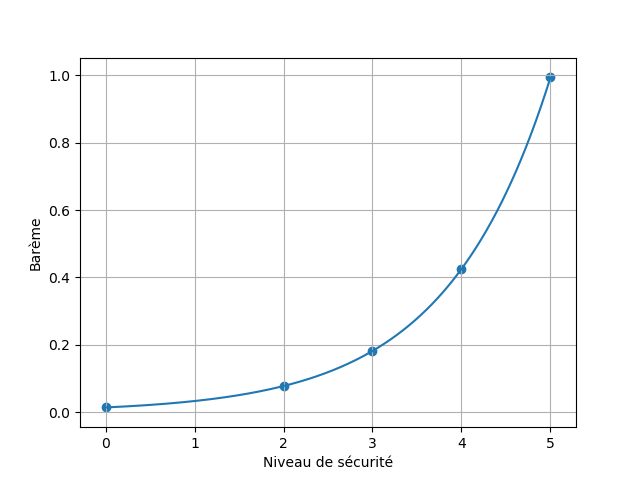
\includegraphics[width=\linewidth]{fig/Securite.png}
%    \caption{Illustration du barème du système de sécurité}
%    \label{fig:bareme_securite}
%\end{wrapfigure}

La résolution du capteur est un aspect important du projet. En effet, une pondération de 10$\%$ lui est attribuée puisque cette caractéristique aura un impact direct sur la capacité de reconnaissance ainsi que sur la qualité des vignettes dans la base de données. Le barème a été conçu à partir d'une fonction exponentielle puisque la différence entre 2 capteurs de résolution inférieure à 8 Mpx doit être significative selon le barème. À l'inverse, en comparant deux capteurs ayant des résolutions supérieures à environ 10 Mpx, la différence importe peu puisque la résolution est jugée suffisante pour les besoins du projet. Puisque les vignettes doivent avoir une taille de 100 par 100 pixels minimalement, la résolution minimale admissible est de 10000 px. Pour trouver la fonction du barème, il a été jugé qu'une résolution de 12 Mpx donnait une note de 0.8 au barème, puisqu'il s'agit d'une résolution suffisante pour le projet.

\begin{equation}
    y = \begin{cases}
        - e^{-0.134(x-0.01)}+1 &  \text{ si } x \geq 0.01 \\
        \text{Rejeté} & \text{ si } x < 0.01
        \end{cases}
    \label{eq:bareme_res}
\end{equation}
où $x$ est la résolution du capteur en Mpx.

\begin{figure}[!htb]
    \centering
    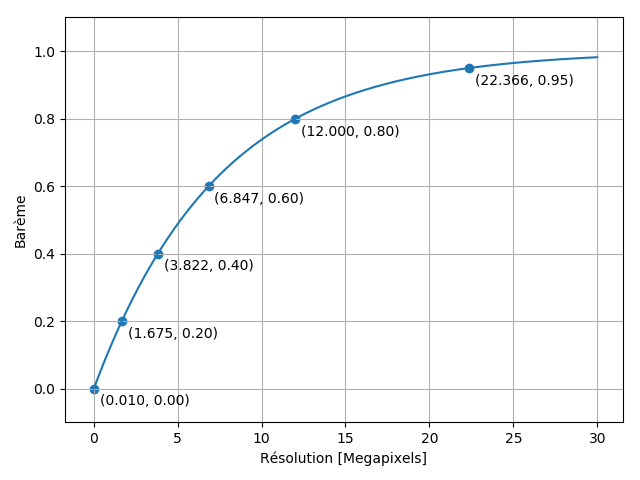
\includegraphics[width=0.45\linewidth]{fig/bareme_resolution.png}
    \caption{Barème pour la résolution du capteur}
    \label{fig:bareme_resolution}
\end{figure}



\subsection{Identification des poissons}

\begin{figure}[!htb]
    \centering
    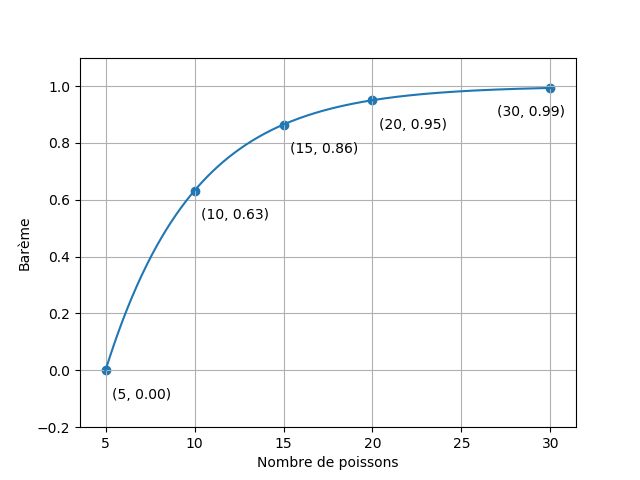
\includegraphics[width=0.45\linewidth]{fig/bareme_identification.png}
    \caption{Barème pour le nombre de poissons à identifier}
    \label{fig:bareme_identification}
\end{figure}

La quantité de poissons reste également à considérer dans l'implantation du système dans la mesure où deux sites différents peuvent chacun comporter une faune aquatique distinctive. Une optimisation de la taille de la librairie des poissons est d'une grande importance lors de la collecte des données par l'appareil: ce dernier doit évidemment être en mesure d'effectuer une bonne reconnaissance du type de poisson. On donnera donc à cette session une pondération de 10\%. Une variété de poisson trop stricte de la librairie causerait une collecte de données erronées dans certain milieux. Il est aussi à noter que le nombre de poissons à considérer est de cinq par site. On définira une équation exponentielle pour la gradation de ce barème: la clé du succès de ce critère repose dans la maximisation du nombre de poisson reconnaissables par la caméra. Par contre, on accordera graduellement moins d'importance à ce critère si le logiciel accepte déjà une grande quantité d'espèces marines. Avec un tel barème, on peut ainsi assurer la compatibilité du logiciel pour son implantation dans différents sites où la faune aquatique pourrait varier.

\begin{equation}
    y(x) = \begin{cases}
        -e^{-0.2(x-5)} + 1 & x \geq 5 \\
        \text{Rejeté} & \text{ si } x < 5 
    \end{cases}
    \label{eq:bareme_identification}
\end{equation}

\subsection{Volume d'imagerie}

Le volume d'imagerie est le volume dans lequel il est possible de prendre des mesures. Plus celui-ci est grand, plus il y de chance qu'il y aura un poisson et plus il sera facile de récolter les mesures. C'est pourquoi il est dans notre intérêt de le maximiser.

Selon les demandes du MFA, le volume minimal d'imagerie doit être de 1m$^3$. Le barème a la forme d'une fonction exponentielle puisqu'il permet d'inclure les systèmes  qui peuvent imager des objets très lointains, ce qui donnerait un volume d'imagerie infini. De plus, à partir de 5m$^3$, le volume d'imagerie est assez grand et avoir un volume d'analyse plus grand n'offre plus un avantage significatif. La fonction a été trouvée à partir des deux points $(1, 0)$ et $(5, 0.8)$.

\begin{equation}
y(x) = \begin{cases}
        -e^{-0.4024(x-1)}+1 & \text{ si } x \geq 1\\
        \text{Rejeté} & \text{ si } x < 1
    \end{cases}
    \label{eq:bareme_volume_analyse}
\end{equation}


\subsection{Capacité de stockage des données}
\label{subsection:capacite_stockage}

La collecte de données est un aspect primordial dans l'énonciation des critères imposés par le ministère: il est impératif que la taille de stockage puisse accepter des données allant jusqu'à une période de deux ans, et ce, à des fins de vérification. Le capteur peut avoir une résolution variant de 0 à 40 Mpx. Par contre, plus de pixels signifie moins de signal par pixel et il ne faut pas oublier que le capteur doit être capable d'opérer la nuit. Ainsi, on considère que la meilleure résolution soit de 12 Megapixels. En supposant que le système stockera en mémoire environ 20 photos par jour pendant 2 ans et que la taille d'un fichier serait de 12$\cdot 10^6$ octets, la capacité minimale de l'espace de stockage devra être de 175 Go. On arrondit ce chiffre à 200 Go pour être conservateur puisqu'il s'agit d'une estimation et que l'on stocke d'autres données supplémentaires comme la température et l'heure. On estime ensuite qu'un système pouvant enregistrer jusqu'à 1000 Go aura une note de 0.8. En utilisant un barème sous la forme exponentielle, on obtient l'équation \ref{eq:bareme_stockage}.

\begin{equation}
    y(x) = \begin{cases}
        -1.5e^{-0.002012x} + 1 & x \geq 200  \\      \text{Rejeté} & \text{ si } x < 200
    \end{cases}
    \label{eq:bareme_stockage}
\end{equation}


\subsection{Durée de vie de l'alimentation du système}

Dans l'objectif d'atteindre une autonomie minimale de deux semaines, il est nécessaire d'optimiser le système d'alimentation du capteur. % De plus, afin de ne pas limiter la disponibilité du capteur, il est idéal d'utiliser une batterie à cet effet. Une batterie rechargeable permettrait également d'augmenter significativement la durée de vie du capteur optique.
La durée de vie minimale demandée est de deux semaines. On considère que la composante chargée d'alimenter le système a une note de 0.8 si celui-ci est en mesure d'accomplir deux cycles de 14 jours. De cette manière, l'opérateur possède un cycle additionnel en cas d'oubli de rechargement. L'autonomie de la durée de vie de l'alimentation est évaluée selon l'équation \ref{eq:bareme_duree_batterie}. Si le système ne peut fournir de l'alimentation au capteur pour une durée de 14 jours, celui-ci sera rejeté.

\begin{equation}
    y(x) = \begin{cases}
        -6.25 e^{-0.13089x}+1 & \text{ si } x \geq 14\\
        \text{Rejeté} & \text{ si } x < 14
    \end{cases}
    \label{eq:bareme_duree_batterie}
\end{equation}


\subsection{Acheminement des informations}

Le système doit être capable de fonctionner à des profondeurs pouvant atteindre les 15.25m sous l’eau. En estimant qu'un poste de contrôle se situe au maximum à 50m de la position du capteur au niveau de l'eau, la distance minimale pour acheminer les données serait d'environ 53m. Puisque le lac le plus profond a une profondeur d'environ 280m~\cite{Lac_walker}, On estime que le critère sera pleinement rempli si le système peut acheminer les données jusqu'à 284m. Ainsi, nous évaluerons ce critère selon l'équation \ref{eq:bareme_acheminement_infos} en utilisant le barème suivant avec $x$ comme étant la distance qui sépare le poste de contrôle local et le système en mètres (m). Si le système ne peut acheminer les informations au-delà de 53m, il sera rejeté automatiquement.

\begin{equation}
    y(x) = \begin{cases}
        \frac{x}{231} - \frac{53}{231} & \text{ si } 53 \leq x \leq 284\\
        \text{Rejeté} & \text{ si } x < 53
    \end{cases}
    \label{eq:bareme_acheminement_infos}
\end{equation}


\subsection{Fiabilité du système de sécurité}

%\begin{wrapfigure}{R}{6cm}
%    \centering
%    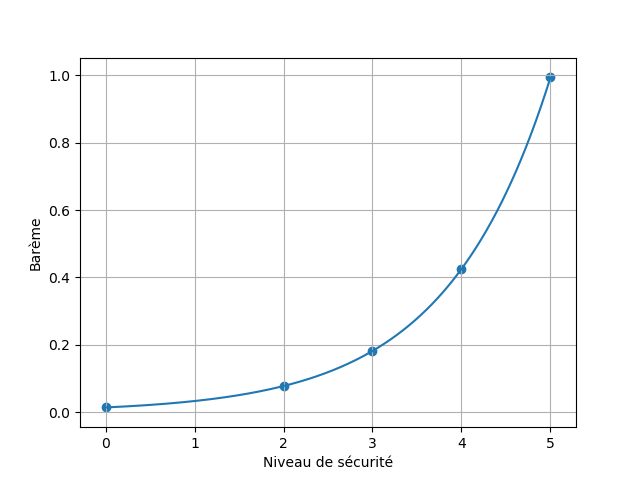
\includegraphics[width=\linewidth]{fig/Securite.png}
%    \caption{Illustration du barème du système de sécurité}
%    \label{fig:bareme_securite}
%\end{wrapfigure}

La confidentialité et l'authenticité des données est primordiale dans un tel projet: c'est pourquoi une grande partie de la cote associée à la qualité du design dépendra de la sécurité du produit. C'est pourquoi un 5\% de la note sera accordée à la sécurité. Plusieurs protocoles de conservation et de transfert des données devront être mis en place, et ce seront justement ici le nombre et la qualité des couches de sécurité offertes par le produit qui permettront une véritable quantification de ce critère. Puisque le système à livrer est fortement axé sur l'autonomie et l'accès à distance, un système qui est facilement compromis est à proscrire à tout prix. Une fonction exponentielle représente parfaitement l'enjeu ici: la moindre faiblesse du système de sécurité peut rendre le produit complètement inutilisable. Le niveau de sécurité $x$ est une combinaison du nombre de couches de sécurité pondéré par leurs qualités respectives.

\begin{equation}
    y = 0.849 e^{0.014x}
    \label{eq:bareme_sécurité}
\end{equation}

\subsection{Résistance à la profondeur du capteur}

La pondération attribuée à ce critère est de 2\%. Le MFA demande un capteur submersible jusqu'à 15.25m de profondeur au minimum. Sachant que le lac le plus profond au Québec est le Lac Walker avec une profondeur de 280m \cite{Lac_walker}, il est possible de déterminer un barème linéaire entre 15.25 et 280m tel que présenté à l'équation \ref{eq:bareme_profondeur}.

\begin{equation}
y(x) = \begin{cases}
        0.003777x-0.0557 & \text{ si } x \geq 15.25\\
        \text{Rejeté} & \text{ si } x < 15.25
    \end{cases}
    \label{eq:bareme_profondeur}
\end{equation}
où $x$ est la profondeur maximale à laquelle le capteur peut être submergé en mètres.

\subsection{Plage de température opérationnelle du capteur}

Une pondération de 2\% est attribuée à ce critère. Le MFA demande que le capteur opère dans une plage de +5°C et -10°C par rapport à l'eau. La température de l'eau peut varier de 4 à 25°C. Le capteur doit donc être opérationnel entre -6 et 30°C. Le barème pour ce critère est montré à la table \ref{t:bareme_resistance_temperature}.

\begin{table}[htp]
   \footnotesize
   \centering
   \begin{tabular}{|c|c|}
        \hline
        Résistance à la température & Barème\\
        \hline
        \hline
        Le capteur est opérationnel sur la plage de -6° à 30°C & 1.0 \\
        \hline
        Le capteur n'est pas opérationnel sur la plage de -6° à 30°C & Rejeté \\
        \hline
   \end{tabular}
   \caption{Barème de la plage de température opérationnelle du capteur}
   \label{t:bareme_resistance_temperature}
\end{table}


\subsection{Taille maximale des spécimens observables}

La pondération attribuée à ce critère est de 4\%. Le MFA demande de pouvoir imager des espèces qui ont une taille minimum de 6 cm. Ça veut dire qu'il faut être capable d'imager des poissons d'au minimum 6cm, mais c'est mieux si il est possible d'imager encore plus petit. Le barème à l'équation \ref{eq:bareme_taille_poisson} est établie selon une fonction exponentielle entre 0 et 6 cm puisqu'une différence entre 0.1 cm et 0.6 cm vaut moins qu'une différence entre 5 et 5.5 cm. Le barème est présenté à l'équation \ref{annexe:bareme_exp_poisson} où les paramètres $a$ et $b$ sont ajustés pour avoir la forme de courbe voulue.

\begin{equation}
y(x) = \begin{cases}
        \frac{1-10^{\frac{x-6}{6}}}{1-10^{-1}} & \text{si } x \leq 6\\
        \text{Rejeté} & \text{ si } x < 6
    \end{cases}
    \label{eq:bareme_taille_poisson}
\end{equation}
où $x$ est la taille minimale des spécimens observables en cm.

% Le capteur optique doit posséder une masse inférieure à 5kg sous l'eau. Le volume du capteur sous l'eau se doit de ne pas dépasser 0.3m$^{3}$. Le capteur doit être fonctionnel jusqu'à une profondeur de 50 pieds. Le système doit supporter une température entre +5°C et -10°C par rapport à la température de l'eau où le capteur sera situé.


\subsection{Nombre de fonctionnalités reliées à l'alarme}

La pondération associée à ce critère est de 2\%. En cas de problème au niveau du transfert de donnée ou de l'opération du capteur, le système doit envoyer une alarme à un responsable. Le nombre de fonctionnalités reliées à l'envoie de l'alarme différencie la qualité entre chaque concept d'alarme. Le dispositif de génération d'alarme doit avoir au minimum 1 fonctionnalité d'alarme. Il est convenu qu'au delà de 10 fonctionnalités, les concepts deviennent équivalents et qu'ils ont une note de 1. Le barème est présenté à l'équation \ref{eq:bareme_etat_systeme}.

\begin{equation}
    y(x) = \begin{cases}
    \frac{x-1}{9} & \text{ si } x \leq 10\\
    1 & \text{ si } x \geq 10\\
    0 & \text{ si } x < 1
    \end{cases}
    \label{eq:bareme_etat_systeme}
\end{equation}
où $x$ est le nombre de fonctionnalités reliées à l'alarme.

\subsection{Puissance de calcul}

La pondération de ce critère est de 2\%. La puissance de calcul sera déterminée par la performance de la carte graphique (source). Le barème est construit à partir d'un score qui reflète la vitesse moyenne effective de la carte graphique \cite{User_Benchmark_score}. La meilleure carte graphique a un score de 219 alors une note de 1 lui sera attribuée. Le barème sera établi de manière linéaire tel que montré à l'équation \ref{eq:bareme_gpu}.

\begin{equation}
    y = \frac{x}{219}
    \label{eq:bareme_gpu}
\end{equation}

\subsection{Utilisation de l'interface graphique}

\begin{table}[htb!]
   \footnotesize
   \centering
   \scalebox{0.8}{
   \begin{tabular}{|c|c|}
        \hline
        Difficulté de l'utilisation de l'interface & Barème \\
        \hline
        \hline
        Très facile & 1.0 \\
        \hline
        Facile & 0.8 \\
        \hline
        Intermédiaire & 0.6 \\
        \hline
        Difficile & 0.4 \\
        \hline
        Très difficile & 0.0 \\
        \hline
   \end{tabular}}
   \caption{Évaluation du barème de l'interface graphique}
   \label{t:bareme_interface}
\end{table}

Puisque l'optique principale de ce projet tourne autour une automatisation des tâches, l'aisance d'utilisation de l'interface lors de l'accès aux données et des opérations de maintenance bimensuelles rejoint tout autant la ligne directrice du design d'appareil (pondération de 5\%). La différenciation entre un interface graphique excellent et médiocre étant difficile à quantifier par calcul, on donnera un barème sous forme de charte, où la valeur la plus grande sera accordée à une qualification de "très intuitive" et la plus faible à "très difficile d'utilisation". La charte des barèmes est présentée à la table \ref{t:bareme_interface}. 


\section{Offrir un système performant}
La performance est un aspect important du projet. Cette section comprend des critères de précision afin d'assurer la performance du système. Une pondération de 20\% est attribué à l'ensemble des critères.

\subsection{Précision du logiciel de reconnaissance}

% \begin{wrapfigure}{R}{7cm}
\begin{figure}[htb!]
    \centering
    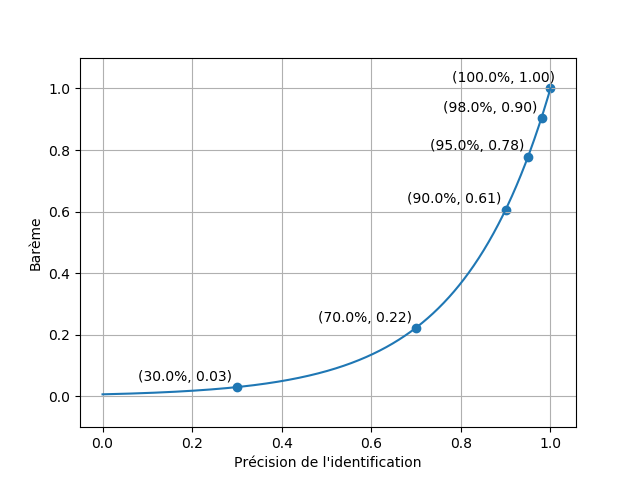
\includegraphics[width=0.45\linewidth]{fig/bareme_ident.png}
    \caption{Illustration du barème pour la précision de l'identification des poissons}
    \label{fig:bareme_precision}
\end{figure}
% \end{wrapfigure}

Le logiciel de reconnaissance du poisson étant au coeur du projet de conception, on donnera une certaine importance à la précision et l'exactitude du programme pour assurer une collecte de données efficace (pondération de 15\%). De plus, un logiciel incapable de faire une bonne différenciation des espèces de poissons ruine l'ensemble des investissements ultérieurs: une excellente caméra ne vaut rien sans un logiciel de qualité. Par contre, à une différenciation d'exactitude dans les très hauts pourcentages (85 à 100), on donnera graduellement moins d'importance aux variations d'efficacité. À un tel niveau d'exactitude, on laissera plus d'importance aux autres caractéristiques en considérant la précision de l'appareil déjà pratiquement maximisée. La fonction quantifiant la qualité de la reconnaissance du poisson s'apparente à une fonction de type exponentielle tel que présenté ci-contre:

\begin{equation}
    y = e^{5(x-1)}
    \label{eq:bareme_precision}
\end{equation}

\subsection{Précision de la température régulée}

La pondération attribuée à la précision de la régulation de la température est de 2$\%$. Le barème prend une forme exponentielle puisqu'un changement de précision près de 1$\%$ d'écart entraîne une plus grosse variation du barème qu'un écart autour de 50$\%$ d'écart. Les paramètres de la fonction exponentielle sont ajustés de manière à ce qu'un pourcentage d'écart de 0$\%$ donne 1 et un pourcentage d'écart de 50$\%$ donne 0.2.

\begin{equation}
    y(x) = e^{-0.03219x}
    \label{eq:bareme_regul}
\end{equation}
où $x$ est la pourcentage d'écart entre la température du système en régime permanent et la température désirée. Il s'agit donc d'un pourcentage d'erreur statique.

\subsection{Précision de la mesure de température}

La pondération attribuée à la précision de la régulation de la température est de 2$\%$. Le barème est basé sur une fonction exponentielle puisqu'il est généralement facile d'avoir une bonne précision pour mesurer la température. L'ajustement des paramètres est le même qu'à l'équation \ref{eq:bareme_regul} pour la régulation de la température.

\begin{equation}
    y(x) = e^{-0.03219x}
    \label{eq:bareme_precision_temperature}
\end{equation}
où $x$ est le pourcentage d'écart entre la température mesurée et la température réelle.

\subsection{Précision de la mesure du temps}

La pondération attribuée à la précision de la mesure du temps est de 1$\%$. Le barème est basé sur une fonction exponentielle puisqu'il prend en compte les très grandes erreurs sur la date et l'heure. L'ajustement des paramètres est fait de manière à ce qu'un écart nul donne une note de 1 et qu'un écart de 2 semaines ($1.2\cdot 10^6$s) donne une note de 0.2.

\begin{equation}
    y(x) = e^{-1.341\cdot10^{-6}x}
    \label{eq:bareme_precision_temps}
\end{equation}
où $x$ est l'écart absolue entre l'heure mesurée et l'heure réelle en secondes.

\section{Coûts}

Une limite des coûts a été établie : on ne peut dépasser 10 000 dollars de frais matériel et 40 000 dollars de coûts de main d'oeuvre. 

Le barème est fait de telle sorte qu'un budget alloué utilisé dans son entièreté donne une note de 0 dans le but de minimiser les coûts. À l'opposé, un coût nul offrirait une note de 1.

Ainsi, de manière générale, le barème pour un tel critère serait:

\begin{equation}
    y(x)=\frac{-x}{\text{Budget}} + 1
\end{equation}

\subsection{Coûts en main d'oeuvre}

\begin{equation}
y(x) = \begin{cases}
        \frac{-x}{40000} + 1 & \text{ si } x \leq 40000\\
        \text{Rejeté} & \text{ si } x > 40000
    \end{cases}
    \label{eq:bareme_cout_logiciel}
\end{equation}

\subsection{Coûts de conception du produit}

La première étape précédant l’utilisation de la machine, est sa conception. Cette partie est non négligeable dans le processus d’analyse des coûts de la machine car elle représente la plus grande source de dépense en matériaux. Afin de combler les besoins du Ministère, on cherche à minimiser les coûts totaux liés à la fabrication de la machine. %En parallèle, il faut limiter les coûts pour que le Ministère puisse économiser et favorisera ainsi le projet.
Ainsi, la fonction décrivant l’efficacité par rapport au coût de production suit une forme suivante :

\begin{equation}
y(x) = \begin{cases}
        \frac{-x}{10000} + 1 & \text{ si } x \leq 10000\\
        \text{Rejeté} & \text{ si } x > 10000
    \end{cases}
    \label{eq:bareme_cout_materiel}
\end{equation}

Un système ne respectant pas la limite de 10000\$ en coûts de matériel sera rejeté. Considérant l'importance du respect des coûts de conception, une pondération de 4\% a donc été attribué à ce critère.


%\section{Respect des contraintes}

%Afin que le concept de solution soit intéressant pour le client, il est nécessaire que chacun des critères concernant les mesures physiques soient respectés. Les critères présent dans cette section représente de nombreux besoins du client. Ainsi, une pondération de 15\% y est attribué. 

%\subsection{Prise de mesure passive}

%Bien que l'objectif principal du capteur est d'identifier une variété de poissons dans un milieu aquatique, il est nécessaire que cette identification n'affecte pas le mode de vie des poissons. En effet, l'une des principales motivations du client à l'égard du projet Fish \& Chips est d'assurer une mesure passive. Le capteur optique ne doit en aucun cas perturber l'environnement des poissons évoluant sur le site. Une importance relative de 2\% est donc accordée à ce critère. En cas de perturbation de l'environnement, le design est automatiquement rejeté, comme le précise la table \ref{t:bareme_systeme_passif}.

%\begin{table}[htp]
%   \footnotesize
%   \centering
%   \begin{tabular}{|c|c|}
%        \hline
%        Degré de passivité du système & Barème\\
%        \hline
%        \hline
%        Le système assure une mesure passive & 1.0 \\
%        \hline
%        Le système n'assure pas une mesure passive & Rejeté \\
%        \hline
%   \end{tabular}
%   \caption{Évaluation du barème du degré de passivité du système}
%   \label{t:bareme_systeme_passif}
%\end{table}

% \subsection{Contraintes mécaniques}

% Le capteur optique doit respecter certaines contraintes physiques et mécaniques. Le non respect de ces contraintes ne doit en aucun cas affecter les fonctionnalités du système. De plus, l'aspect physique du capteur optique ne doit pas être un facteur pouvant perturber l'environnement des poissons. C'est dans cette optique qu'on attribue aux contraintes mécaniques une pondération de 5\% de l'ensemble du projet. Ce barème a été calculé considérant le tableau \ref{eq:bareme_volume_capteur} et les caractéristiques suivantes:

%\subsection{Masse du capteur}

%Le MFA spécifie que le capteur optique doit posséder une masse inférieure à 5kg sous l'eau. Pour cette raison, un capteur ayant une masse supérieure à 5 kg sera rejeté. Le barème présenté à l'équation \ref{eq:bareme_masse_capteur} prend la forme d'une fonction cosinus pour que le barème ne varie pas beaucoup près de 0 et 5 kg puisqu'un design de capteur ayant une masse de 0 à 1 kg serait très bon et que deux designs de capteur ayant une masse entre 4 et 5 kg seraient presque équivalents. Par contre, le barème varie à peu près linéairement entre 1 et 4 kg. La fréquence du cosinus est ajustée de manière à ce qu'il y ait une demie période entre 0 et 5kg. La pondération attribuée à ce critère est de 2$\%$ étant donné que le plus important est tout simplement d'avoir une masse respectant la demande du client.

%\begin{equation}
%y(x) = \begin{cases}
%        1 & \text{ si } 0 \le x \leq 5\\
%        \text{Rejeté} & \text{ si } x > 5
%    \end{cases}
%    \label{eq:bareme_masse_capteur}
%\end{equation}
%où $x$ est la masse du capteur submergé en kg.

%\subsection{Volume du capteur}


%Selon la demande du client, le volume du capteur doit être inférieur à 0.3 m$^3$. L'équation \ref{eq:bareme_volume_capteur} pour le barème du volume du capteur a la même forme que l'équation \ref{eq:bareme_masse_capteur} pour les mêmes raisons citées ci-dessus. La seule différence est que les paramètres sont ajustés de manière à ce qu'un volume de 0.3m$^3$ donne une note de 0. La pondération attribuée à ce critère est de 2$\%$ puisqu'il est surtout important d'avoir un volume inférieur à 0.3m$^3$.

%\begin{equation}
%y(x) = \begin{cases}
%        1 & \text{ si }0 \le x \leq 0.3\\
%        \text{Rejeté} & \text{ si } x > 0.3
%    \end{cases}
%    \label{eq:bareme_volume_capteur}
%\end{equation}
%où $x$ est le volume du capteur submergé en m$^3$.


%\subsection{Intervalle de température mesurable}


%\begin{equation}
%y(x) = \begin{cases}
%    1 & \text{ si } -6 \leq x \leq 30\\
%    \text{Rejeté} & \text{Autrement}
%    \end{cases}
%    \label{eq:bareme_mesure_temperature}
%\end{equation}


%\begin{enumerate}
%    \item Le capteur optique doit posséder une masse inférieure à 5kg sous l'eau.
%    \item Le volume du capteur sous l'eau se doit de ne pas dépasser 0.3$m^{3}$. 
%    \item Le capteur doit être fonctionnel jusqu'à une profondeur de 50 pieds.
%    \item Le système doit supporter une température entre +5°C et -10°C par rapport à la température de l'eau où le capteur sera situé.
%\end{enumerate}


%   \begin{enumerate}
%       \item Les images capturées doivent être en couleur.
%       \item La taille des images ne doit pas excéder 8 bits.
%       \item Les dimensions des photos doivent être de 100 X 100 pixels.
%       \item Chacune des images recueillies doivent également fournir la date et l'heure, la           température interne du système, la température de l'eau et l'identification du poisson.
%       \item Le capteur optique doit être en mesure d'observer des spécimens de plus de 6cm.
%       \item Le système doit être en mesure de capter des poissons dans un volume minimal de           1$m^{3}$.
%    \end{enumerate}



%\section{Intervention humaine}

%En analysant les demandes du client, on se rend vite compte que l’automatisation du système sera un élément prépondérant dans notre système. Pour parvenir à un système autonome, il faudra impérativement tenir compte de certains aspects comme la  durée de vie de la batterie, l’automatisation des transferts de données, l’accès à distance ainsi que la complexité de la maintenance qu’il faudra minimiser afin de réduire au maximum l’intervention humaine. Compte tenu de l’importance de cet aspect dans le projet, l’équipe de conception attribue une pondération de 20\%.


\newpage


\section{Maison de qualité}

\begin{figure}[htb!]
    \centering
    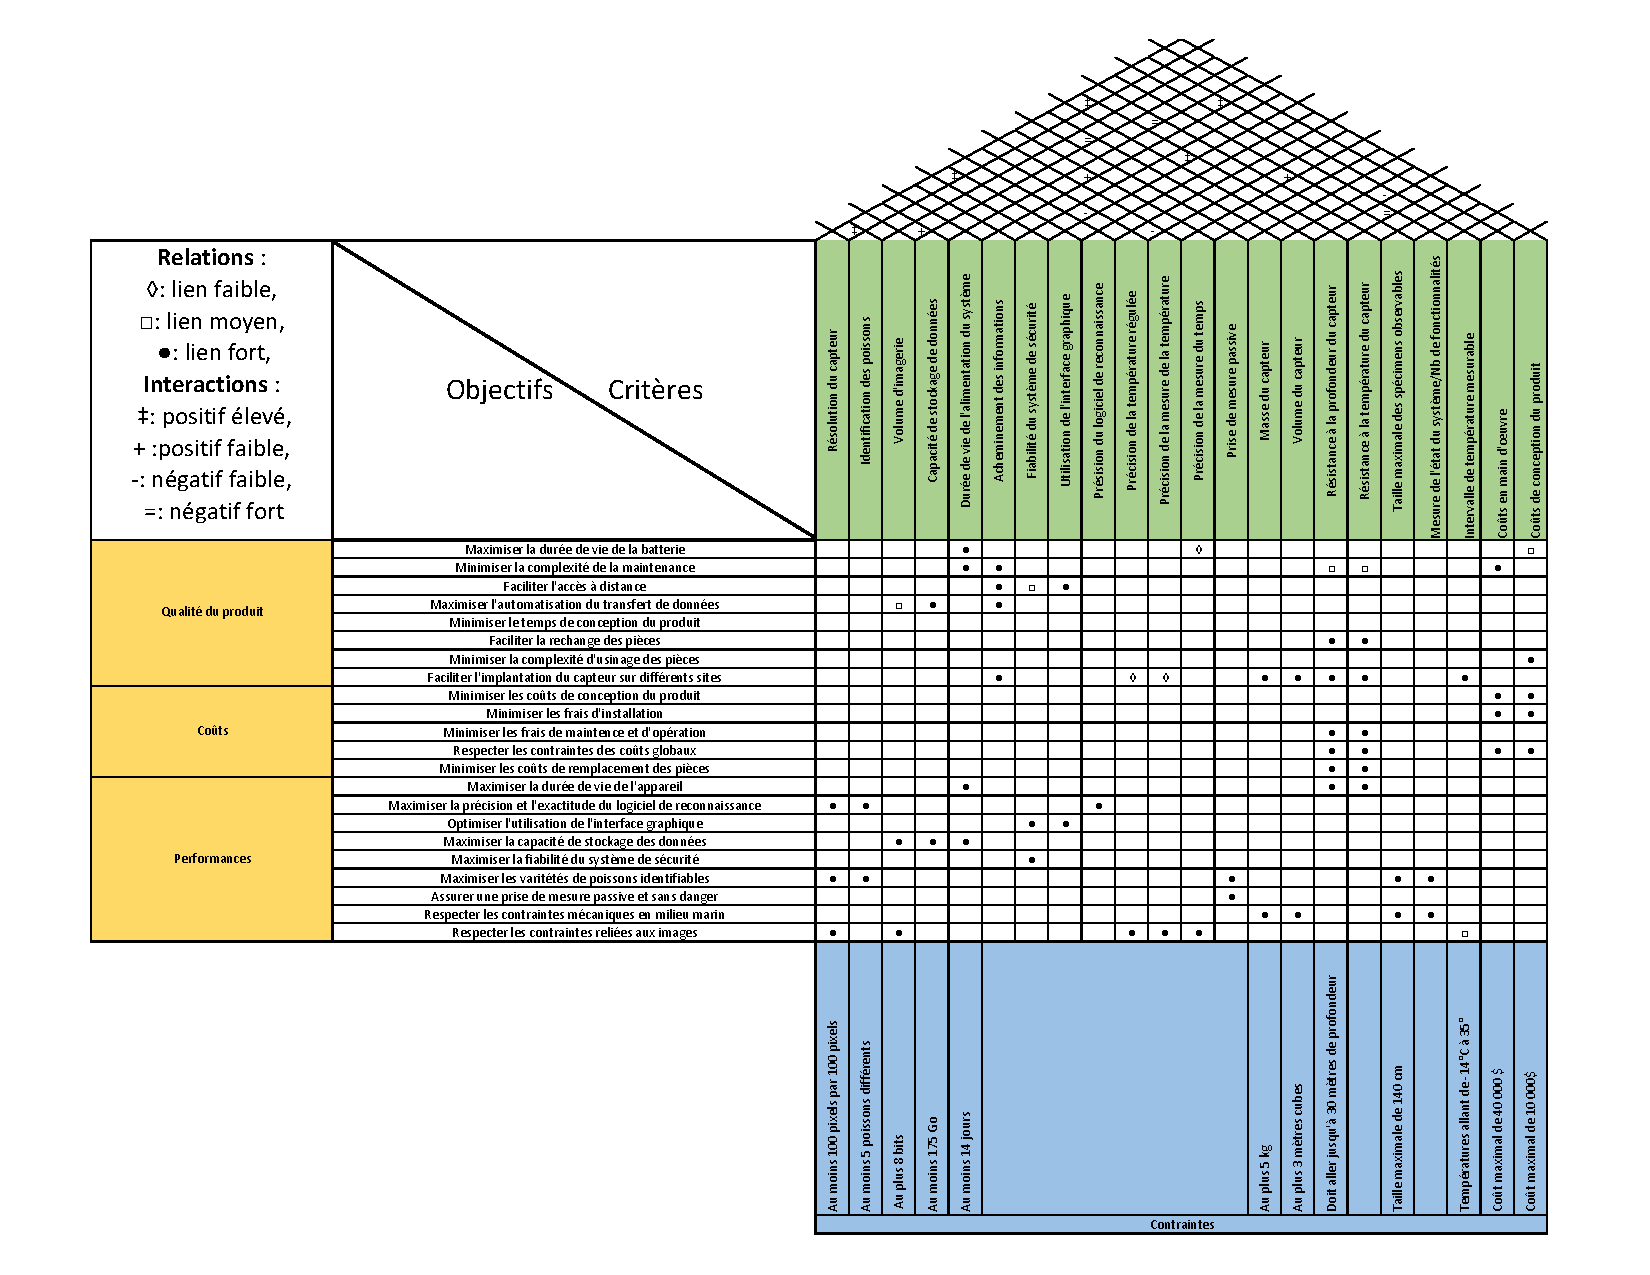
\includegraphics[width=\linewidth]{fig/MQ3.pdf}
    \caption{Maison de qualité du projet Fish \& Chips}
    \label{fig:maison_qualite}
\end{figure}
